\RequirePackage{shellesc}
\immediate\write18{cd ..; tex braids_code.dtx}
\documentclass{article}

\usepackage{tikz}
\usetikzlibrary{
  braids,
  arrows.meta
}

\begin{document}

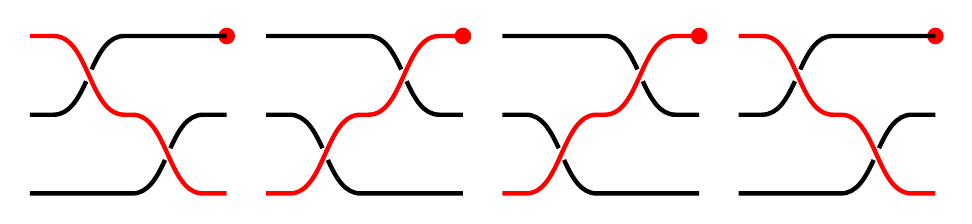
\begin{tikzpicture}[ultra thick]
\fill[red] (1,2) circle[radius=3pt];
\fill[red] (4,2) circle[radius=3pt];
\fill[red] (7,2) circle[radius=3pt];
\fill[red] (10,2) circle[radius=3pt];
\def\braidAnchor{south east}
\pic[
  rotate=90,
  braid/.cd,
  strand 1/.style={red},
  height=1cm,
  width=1cm,
  anchor=\braidAnchor,
] (braid) at (1,2) {braid={s_1 s_2}};
\pic[
  rotate=90,
  braid/.cd,
  strand 1/.style={red},
  height=1cm,
  width=-1cm,
  anchor=\braidAnchor,
] (braid) at (4,2) {braid={s_1 s_2}};
\pic[
  rotate=90,
  braid/.cd,
  strand 1/.style={red},
  height=-1cm,
  width=1cm,
  anchor=\braidAnchor,
] (braid) at (7,2) {braid={s_1 s_2}};
\pic[
  rotate=90,
  braid/.cd,
  strand 1/.style={red},
  height=-1cm,
  width=-1cm,
  anchor=\braidAnchor,
] (braid) at (10,2) {braid={s_1 s_2}};
\end{tikzpicture}


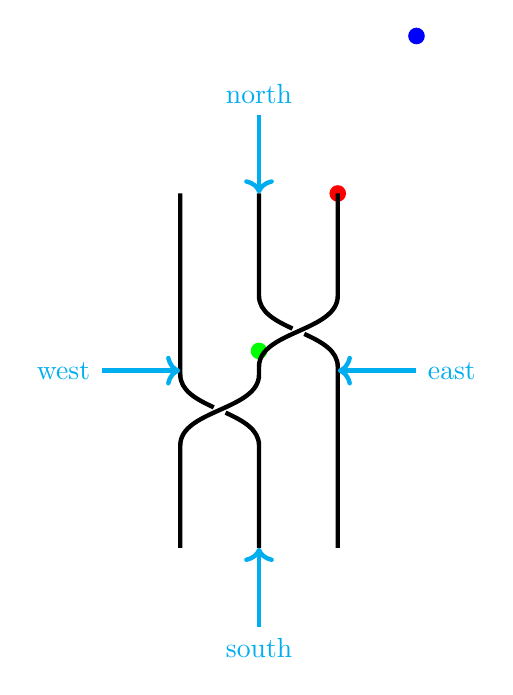
\begin{tikzpicture}[ultra thick]
\fill[red] (1,2) circle[radius=3pt];
\fill[blue] (2,4) circle[radius=3pt];
\fill[green] (0,0) circle[radius=3pt];
\pic[
  braid/.cd,
  height=-1cm,
  width=-1cm,
  anchor=north east,
] (braid) at (1,2) {braid={1 s_1 s_2 1}};
\draw[<-,cyan] (braid.east) -- +(1,0) node[right] {east};
\draw[<-,cyan] (braid.west) -- +(-1,0) node[left] {west};
\draw[<-,cyan] (braid.north) -- +(0,1) node[above] {north};
\draw[<-,cyan] (braid.south) -- +(0,-1) node[below] {south};
\end{tikzpicture}


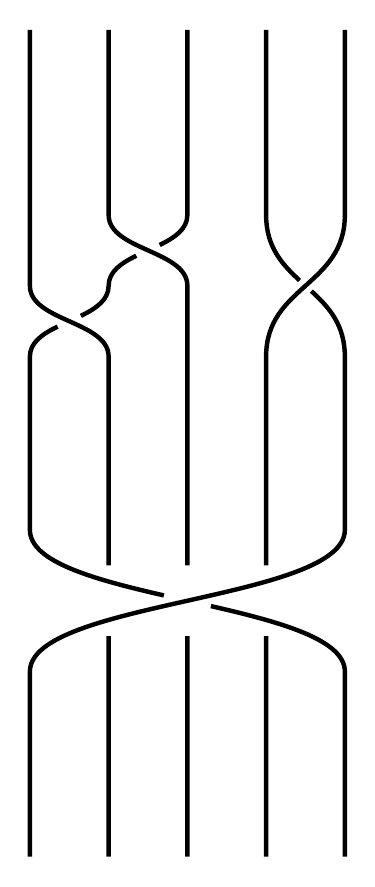
\begin{tikzpicture}[ultra thick]
\pic[
  braid/.cd,
  height=2cm,
%  nudge factor=0.25,
]
{braid={1 s_{1,5} 1 s_{1,2,3}^{-1}-s_4 1}};
\end{tikzpicture}



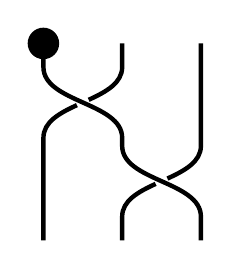
\begin{tikzpicture}[ultra thick]
\pic[name prefix=braid] {braid={s_1 s_2}};
\fill (braid-1-s) circle[radius=2mm];
\end{tikzpicture}


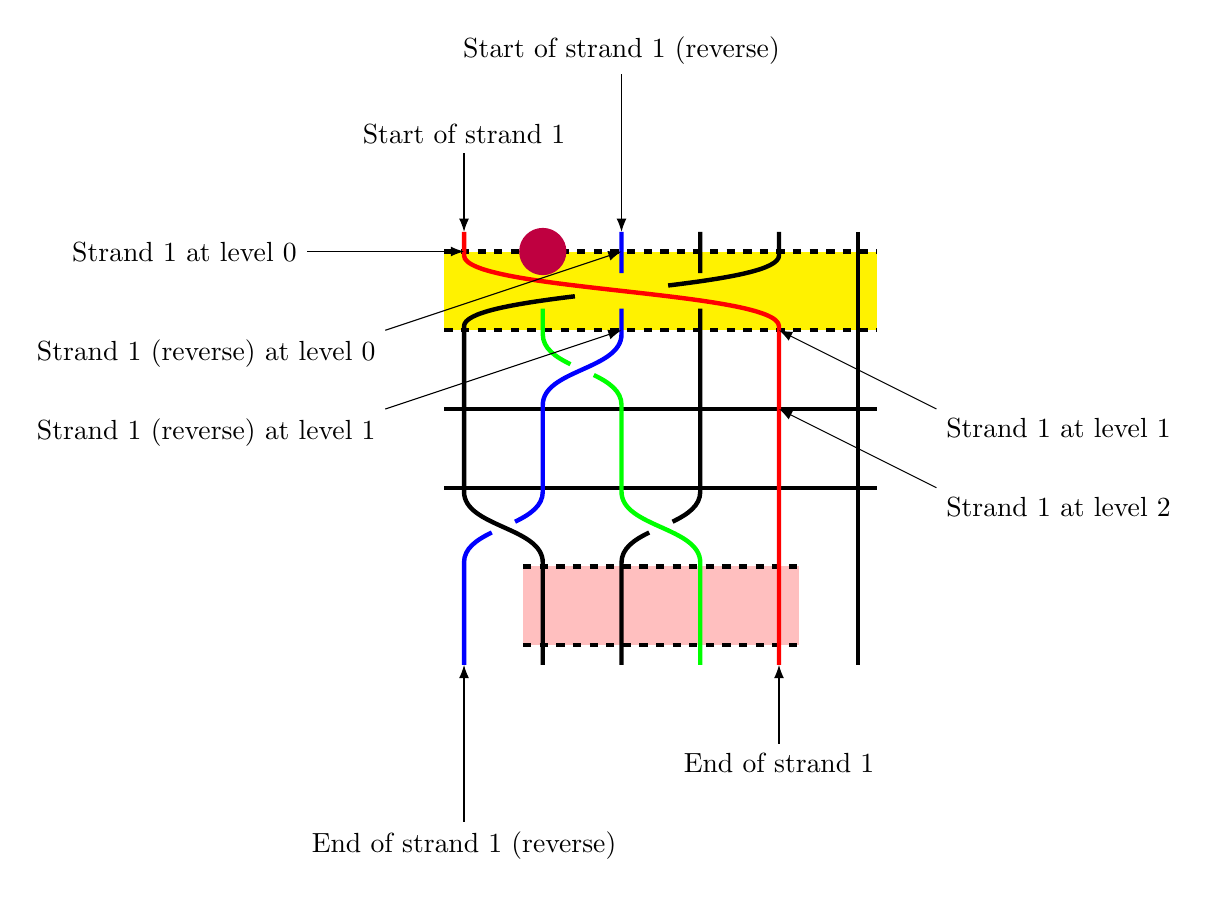
\begin{tikzpicture}[>=Latex]
\pic[
  ultra thick,
  braid/strand 1/.style={red},
  braid/strand 2/.style={green},
  braid/strand 3/.style={blue},
  braid/every floor/.style={draw=black},
  braid/floor 1/.style={fill=yellow,dashed},
  braid/floor a/.style={fill=pink,dashed},
  braid/number of strands=6,
  braid/width=1cm,
  braid/gap=.1,
  braid/anchor=2-0,
  braid/add floor={2,4,3,1,a},
  name prefix=braid,
] {braid={|s_{1,5} s_2^{-1} | 1 s_3-s_1 1}};% s_2 | s_1^{-1}-s_3 | 1 s_1}};
\draw[<-] (braid-1-e) -- +(0,-1) node[below] {End of strand 1};
\draw[<-] (braid-1-s) -- +(0,1) node[above] {Start of strand 1};
\draw[<-] (braid-rev-1-e) -- +(0,-2) node[below] {End of strand 1 (reverse)};
\draw[<-] (braid-rev-1-s) -- +(0,2) node[above] {Start of strand 1 (reverse)};
\draw[<-] (braid-1-2) -- +(2,-1) node[below right] {Strand 1 at level 2};
\draw[<-] (braid-1-1) -- +(2,-1) node[below right] {Strand 1 at level 1};
\draw[<-] (braid-rev-1-1) -- +(-3,-1) node[below left] {Strand 1 (reverse) at level 1};
\draw[<-] (braid-1-0) -- +(-2,0) node[left] {Strand 1 at level 0};
\draw[<-] (braid-rev-1-0) -- +(-3,-1) node[below left] {Strand 1 (reverse) at level 0};
\fill[purple] (0,0) circle[radius=3mm];
\end{tikzpicture}
\end{document}
